\chapter{Organização dos dados}

Os dados utilizados como entrada para esses algoritmos são baseados em séries temporais de valores que representam o comportamento de alguma variável atmosférica, tal como quantidade de chuva e temperatura do ar, num local específico em vários momentos do tempo. Essas informações podem ser obtidas por satélites, balões atmosféricos, estações meteorológicas, entre outros, e normalmente são medidas uma ou mais vezes por dia. A partir da obtenção dessas séries de dados em diversos locais espalhados por uma determinada área, ou até mesmo no globo terrestre inteiro, são feitas verificações para a validação desses valores e executado métodos para a dedução dos valores referentes a localidades onde não é possível fazer a medição, como por exemplo no meio dos oceanos. Enfim é criado uma grade que divide igualmente a área de interesse em pequenas quadrículas, de tal forma que cada uma dessas áreas seja representada por apenas uma série de dados, e de que a visualização como um todo dessas várias séries represente o comportamento da variável em questão na área total. 

Em geral a utilização de apenas uma série de dados para cada uma dessas áreas pode gerar muitas informações equivocadas, uma vez que o comportamento dessas variáveis atmosféricas podem variar bruscamente dentro de cada uma dessas regiões. Por isso há a necessidade de que o tamanho dessas regiões seja o menor possível. Entretanto isso faz com que haja muito mais séries para a mesma área de interesse, o que numa escala global faz com que o número de quadrículas cresça bruscamente.

Existem diversas instituições que fornecem livremente esses dados ao público, como o National Oceanic \& Atmospheric Administration \cite{NOAA} e a NASA \cite{NASA} dos Estados Unidos da América, e o Met Office Hadley Centre \cite{MOHC} do Reino Unido. São dados como esses que servem como base para estudos sobre mudanças climáticas.

\section{Estrutura de dados}

A estrutura de dados usada para armazenar essas informações é uma matriz tridimensional (X,Y,T) na qual os eixos X e Y se referem a posição espacial e o eixo T ao tempo, e cada um desses eixos possui uma quantidade fixa de valores, respectivamente NX, NY e NT. Essa estrutura é armazenada de forma sequencial variando primeiramente os eixos X e Y e por fim o eixo T, ou seja, os valores do eixo T para cada ponto (X,Y) ficam separados.

\section{Tamanho dos dados}

Um dos principais desafios enfrentados no uso desses dados é o tamanho dos arquivos necessários para armazenar toda a informação, que pode ser calculado multiplicando-se o número total de quadrículas (NP = NX * NY) pelo tamanho de cada uma das séries de dados (NT). Por exemplo, para armazenar as informações referentes a 1 ano de valores diários, para uma grade global de 360 por 180 quadrículas são necessários 94608000 bytes (NT=365 x [NX=180 * NY=360] x 4 bytes), ou aproximadamente 90MB. Pode não parecer muito mas, sabendo-se que cada uma dessas quadrículas abrange uma área de aproximadamente 110Km$^2$ e são as informações de apenas 1 ano, percebe-se que para um período de dados um pouco maior ou para quadrículas com uma área um pouco menor esse valor pode chegar facilmente na casa dos GigaBytes. Prova disso é que, para esse mesmo exemplo citado, caso fosse um período de 50 anos seriam necessários 4.4GBs.

%%%%%%%%%%%%%%%%%%%%%%%%%%%%%%%%%%%%%%%%%%%%%%%%%%%%%%%%%%
% FIGURA
\begin{figure}[H]
\centering
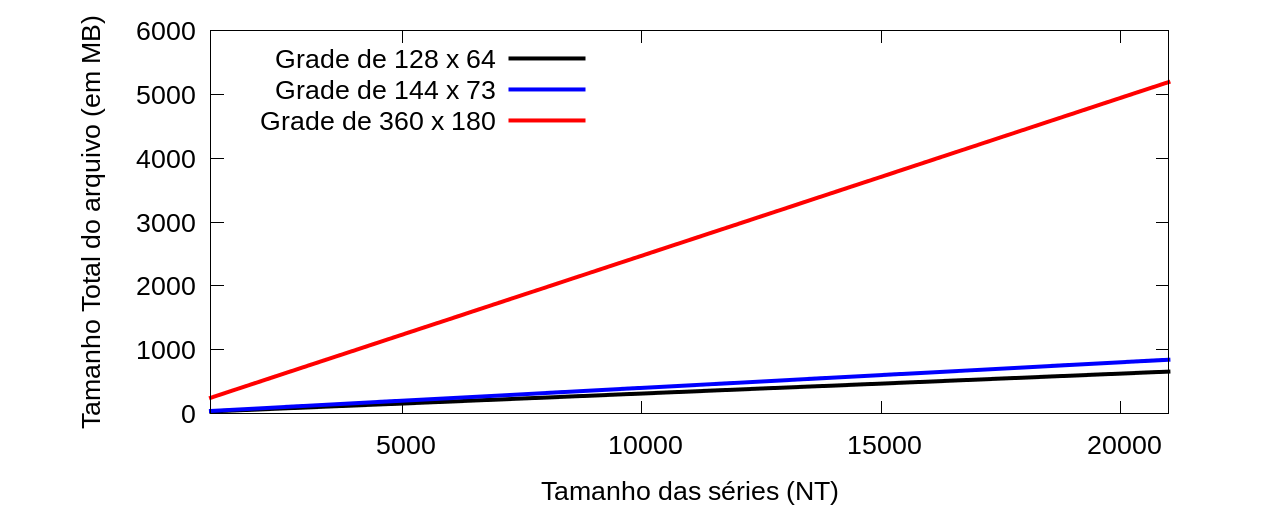
\includegraphics[width=1.0\textwidth]{Imagens/tamanho_dados/serie_tam_dados.png}
\caption{Gráfico do tamanho dos arquivos de dados}
\label{fig:grafico_tamanho_dados}
\end{figure}
%%%%%%%%%%%%%%%%%%%%%%%%%%%%%%%%%%%%%%%%%%%%%%%%%%%%%%%%%%